%Table Head Macro
\newcommand*{\thead}[1]{\multicolumn{4}{|c|}{\bfseries #1}}

\section{Projektmeilensteinplan}
\begin{table}[!h]
\caption{Projektmeilensteinplan}
\centering
\begin{tabular}{|l|l|l|l|}
\hline
\thead{Projektmeilensteinplan} \\
\hline
\hline
PSP-Code & Meilenstein & Plantermin & Isttermin \\ [1ex]
\hline
& Projektstart & 05.10.2013 & \\
\hline
1.3 & Start Recherche & 05.10.2013 & \\
\hline
1.4 & Grobplanung & 05.10.2013 & \\
\hline
1.4.1 & Konzeptions beginn & 21.11.2013 & \\
\hline
1.6 & Modellierung Ende & 06.12.2013 & \\
\hline
1.7.1 & Start Hauptprogramm Entwicklung & 07.12.2013 & \\
\hline
1.7.2 & Beginn Plugin-Entwicklung & 21.12.2013 & \\
\hline
1.8  & Start Testen & 06.12.2013 & \\
\hline
1.9 & Projektabschluss & 10.01.2013 & \\
\hline
\end{tabular}
\end{table}

\section{Projektmeilensteinbalkenplan}
\begin{figure}[!ht]
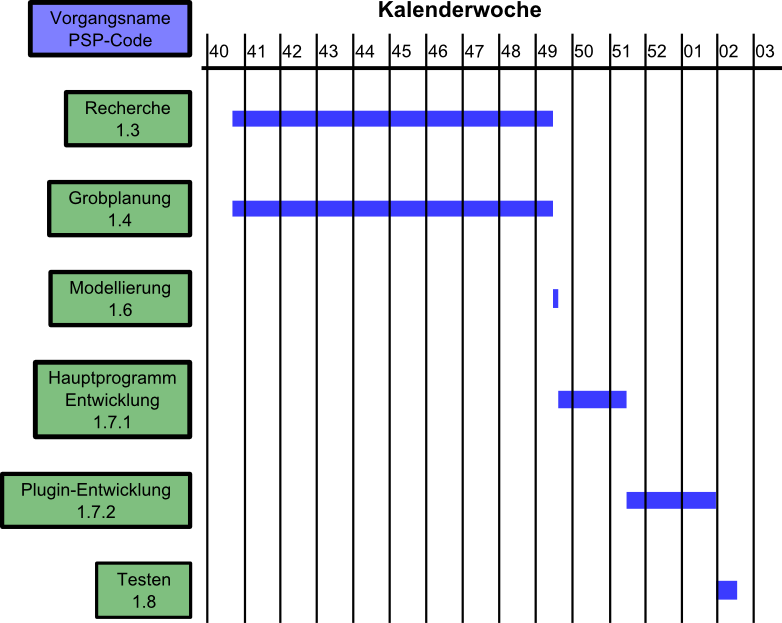
\includegraphics[width=\textwidth, height=\textheight, keepaspectratio, angle=0]{images/balkenplan}
\caption{Balkenplan}
\end{figure}
